\section{Abstract}
In this computer based test we are asked to perform linear regression by least squares on a given data set. The dataset analysed is the Olympic men's running time (100m and 400m) for a given range of years. 

In Task 1 we determine which polynomial function is the best fit for the 400m data. A common validation method is used to ensure the model is competent. In Task 2 we determine the best value of the regularisation factor, $\lambda$, for the polynomial functions of order 1 and 4.

In short, the results of Task 1 illustrate a polynomial function with order 2 best fits the Olympics men's 400m data. In Task 2, the results show a regularisation factor, $\lambda$, with value 0, gives the best predictive performance for both polynomial functions on the Olympic men's 100m data.

The analysis was performed in Matlab, and the code listings can be found in Appendices A and B.

\section{Scope}
The report consists of the following structure.

\begin{enumerate}
	\item Overall Task
		\subitem Details of task set out in the ``Computer Based Test 2.''
	\item Maximum Likelihood (ML)
		\subitem Discussion on training the ML with and without the Naive assumption
		\subitem Interpretation of results
	\item Maximum A Posteriori (MAP)
			\subitem Discussion on training the MAP with and without the Naive assumption
			\subitem Interpretation of results
	\item Maximum Likelihood VS Maximum A Posteriori
			\subitem Difference of ML and MAP
			\subitem Affects of Difference on this data 
\end{enumerate}

\section{Overall Task}
The analysis was performed on a data set of diseased and healthy patients. The data set has been plotted in Figure \#.

\begin{figure}[h]
	\centering
	\includegraphics[width=0.8\linewidth]{images/MLtrainingData}
	\caption{Comparison of the CV and Train loss for polynomial models of order \textbf{n}, where \textbf{n} = 0 to 4.}
	\label{fig:CVT4}
\end{figure}

\section{Maximum Likelihood (ML)}{\label{s1}
	
\subsection{Introduction}\label{Int}
In Task 1, we are asked to analyse the Olympics men's 400m data. We must find the polynomial function of order \textbf{n} which best fits this data, where \textbf{n} is 1 to 4, and use 10-fold cross-validation to choose the "best" value of \textbf{n}. Refer to Appendix A for the Matlab code used for analysis.

To compute the average cross validation loss, data (attributes and labels) are separated into 10 partitions (i.e. 10-fold), where 1 partition is reserved for testing the model. The 9 remaining partitions are used to learn the model with parameters, $w_{n}$. This models can use the attributes of the test partition to predict the labels, in this case the time ran for the men's 400m. The predicted values can then be compared to the actual values (labels)  from the test partition. The cross validation (CV) loss is calculated by taking the mean squared difference ($msd$) of these two values. This is then repeated 9 more times by rotating the test partition through. The average of these 10 $msd$ values is calculated and then plotted against the order to find the minimum value.
\subsection{Results}\label{CVcons}
From Figure \ref{fig:CVT4} and Table \ref{t:ModLoss} it is shown that a polynomial function with order 4 is the best fit. However, in order to determine the "best" order, it must be given a concrete meaning for this task. "Best" is considered to be the minimum mean squared loss, where loss is the difference between predicted and observed labels. Ideally, both cross-validation (CV) and training loss are considered but that is not always the case. So, three cases are defined as the following.

\begin{enumerate}
	\item Only CV loss is considered
	\item Only Train loss is considered
	\item Both CV and Train loss are considered
\end{enumerate}

\begin{figure}[h]
	\centering
	\includegraphics[width=0.8\linewidth]{images/MLnewData}
	\caption{Comparison of the CV and Train loss for polynomial models of order \textbf{n}, where \textbf{n} = 0 to 4.}
	\label{fig:CVT4}
\end{figure}

\begin{figure}[h]
	\centering
	\includegraphics[width=0.8\linewidth]{images/MLWONnewData}
	\caption{Comparison of the CV and Train loss for polynomial models of order \textbf{n}, where \textbf{n} = 0 to 4.}
	\label{fig:CVT4}
\end{figure}

\begin{table}[h]
	\centering
	\caption{Classification Differences between Methods}
	\label{t:ModLoss}
	\begin{tabular}{rrrr}
		\hline
		\textbf{Order} & \textbf{CV Loss} & \textbf{Train Loss} & \textbf{Average Squared Loss} \\ \hline
		0 & 10.83 & 8.07 & 178.61 \\
		1 & 2.71 & 1.54 & 9.03 \\
		2 & 1.57 & 1.01 & 3.33 \\
		3 & 3.99 & 0.98 & 12.35 \\
		4 & 1.64 & 0.93 & 3.30
	\end{tabular}
\end{table}

Consider item 1, Figure \ref{fig:CVT4} and Table \ref{t:ModLoss} show that a polynomial function with order 2 is the best fit. It is visualised clearly on Figure \ref{fig:CVT4} as the minimum point on the line. Looking at Table \ref{t:ModLoss}, a minimum value of 1.57 also corresponds with order 2.

Consider item 2, Figure \ref{fig:CVT4} and Table \ref{t:ModLoss} show that a polynomial function with order 4 is the best fit. Figure \ref{fig:CVT4} shows a downward trend to the right, indicating that an order of 4 is indeed the best fit. Looking at Table \ref{t:ModLoss}, the minimum value, 3.30, also corresponds with an order of 4.

Consider item 3, Figure \ref{fig:CVT4} and Table \ref{t:ModLoss} show that a polynomial function with order 4 is the best fit. It is difficult to see this via the visualisation of Figure \ref{fig:CVT4}. However, looking at Table \ref{t:ModLoss}, the average squared loss (of CV and Train loss) is lowest when order equals 4. 

Figure \ref{fig:model2} shows how well each of the models fit the data. Interestingly, Figure \ref{fig:model4}, shows an order of 4 provides an accurate model and more realistic future predictions than an order of 2. In comparison, an order of 2 shows that future predictions would increase in time at an increasing rate. This is highly unlikely given the downward trend of the data.

The remaining models in Figure \ref{men400-1} clearly do not model the data well, where orders 1 and 3 show that a time of 0 will be achieved soon. This is not humanly possibly so the models can be discarded. 

\subsection{Conclusion}
The problem for Task 1 is to find the "best model based on average cross-validation loss." This only considers point 1 from before, therefore, a polynomial function with order 2 best fits the model based on average cross-validation loss.

\begin{figure}[h!] 
	\centering
	\begin{subfigure}[b]{0.4\textwidth}
		\includegraphics[width=\textwidth]{MLtrainingData.png}
		\caption{Polynomial model with order \textbf{n} = 3}
		\label{fig:modelNoReg0}
	\end{subfigure}
	\begin{subfigure}[b]{0.4\textwidth}
		\includegraphics[width=\textwidth]{MLnewData.png}
		\caption{Polynomial model with order \textbf{n} = 4}
		\label{fig:modelNoReg1}
	\end{subfigure}
	\begin{subfigure}[b]{0.4\textwidth}
	\includegraphics[width=\textwidth]{MLWONnewData.png}
	\caption{Polynomial model with order \textbf{n} = 4}
	\label{fig:modelNoReg1}
	\end{subfigure}
	\caption{The original Olympic men's 400m data (blue crosses) with the polynomial models (red) overlaid without data standardisation.}
	\label{men400-1noSt}
\end{figure}

\subsection{Further Comments}
Further investigation found if the data was not standardised, a systematic error is produced in the model for orders greater than or equal 4. Figure \ref{men400-1noSt} illustrates an order of 3 produces no error, but an order of 4 does. Reviewing literature showed this systematic error is common when dealing with high order polynomial function\cite{WhenIsIt}.Therefore, it is good practice to standardise data when the regression model contains polynomial terms.

\begin{figure}[h!] 
	\centering
	\begin{subfigure}[b]{0.4\textwidth}
		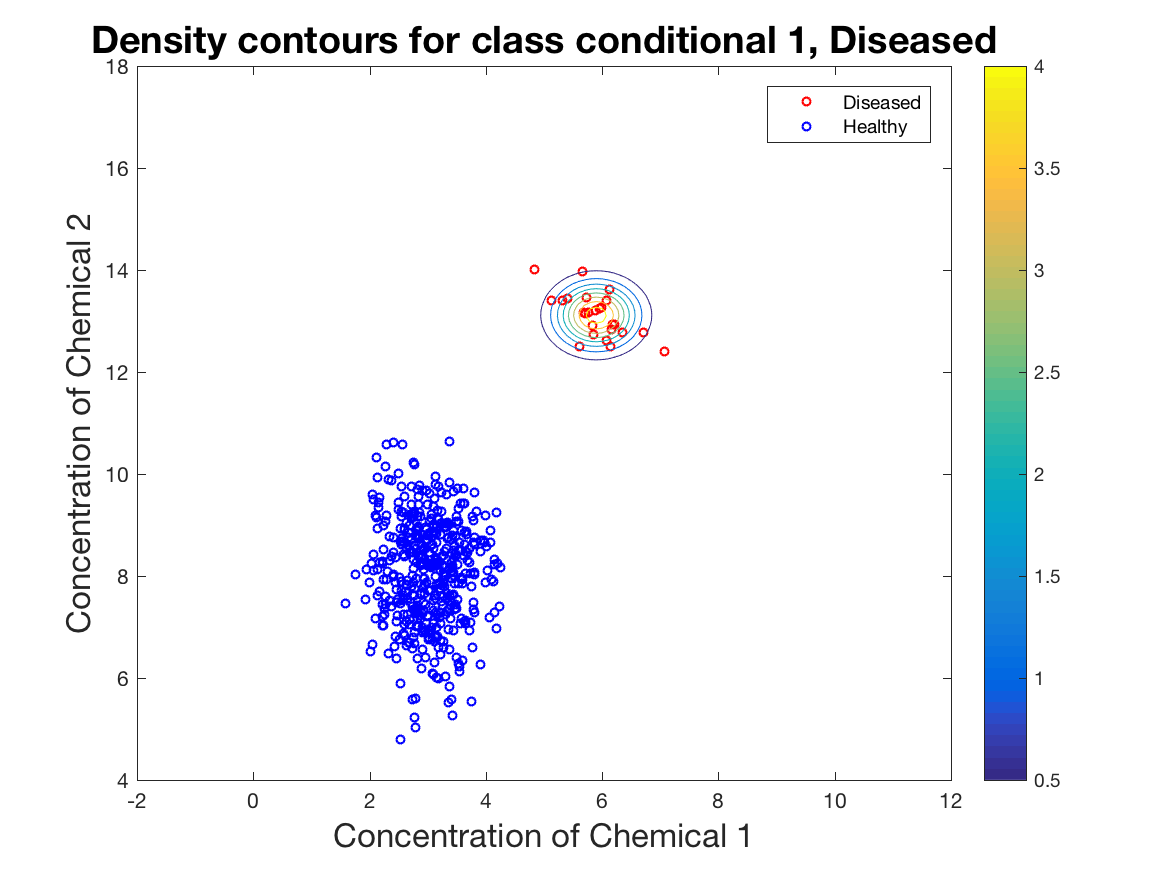
\includegraphics[width=\textwidth]{MLclassCondContoursDiseased.png}
		\caption{Polynomial model with order \textbf{n} = 0}
		\label{fig:model0}
	\end{subfigure}
	\begin{subfigure}[b]{0.4\textwidth}
		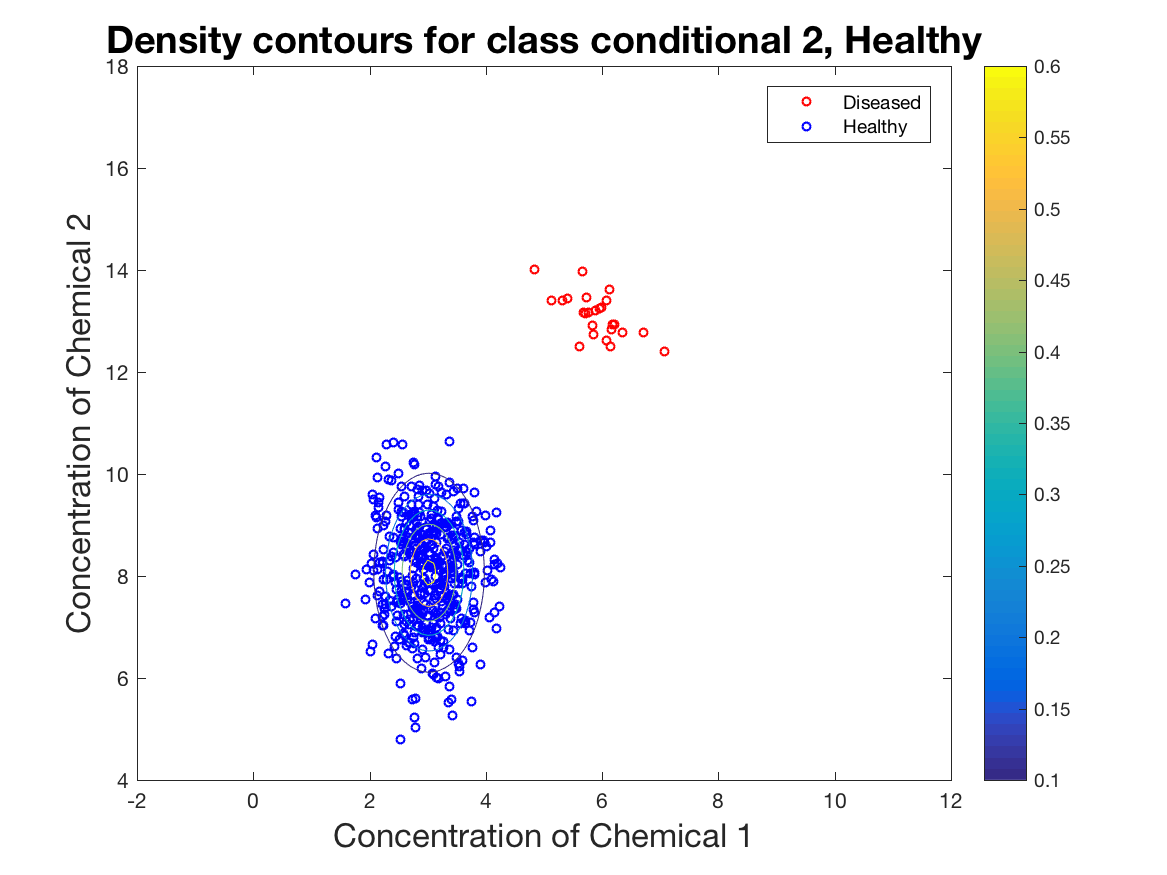
\includegraphics[width=\textwidth]{MLclassCondContoursHealthy.png}
		\caption{Polynomial model with order \textbf{n} = 1}
		\label{fig:model1}
	\end{subfigure}
	\begin{subfigure}[b]{0.4\textwidth}
		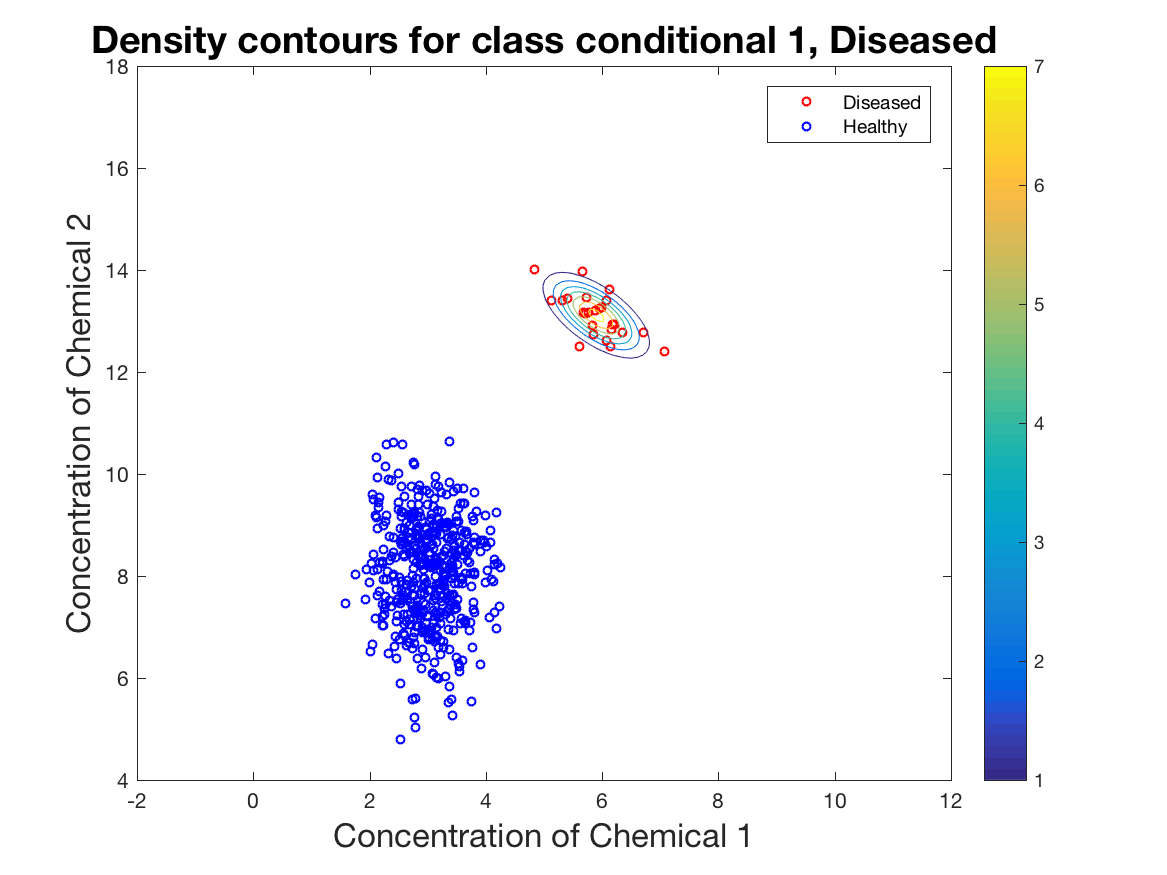
\includegraphics[width=\textwidth]{MLWONclassCondContoursDiseased.png}
		\caption{Polynomial model with order \textbf{n} = 2}
		\label{fig:model2}
	\end{subfigure}
	\begin{subfigure}[b]{0.4\textwidth}
		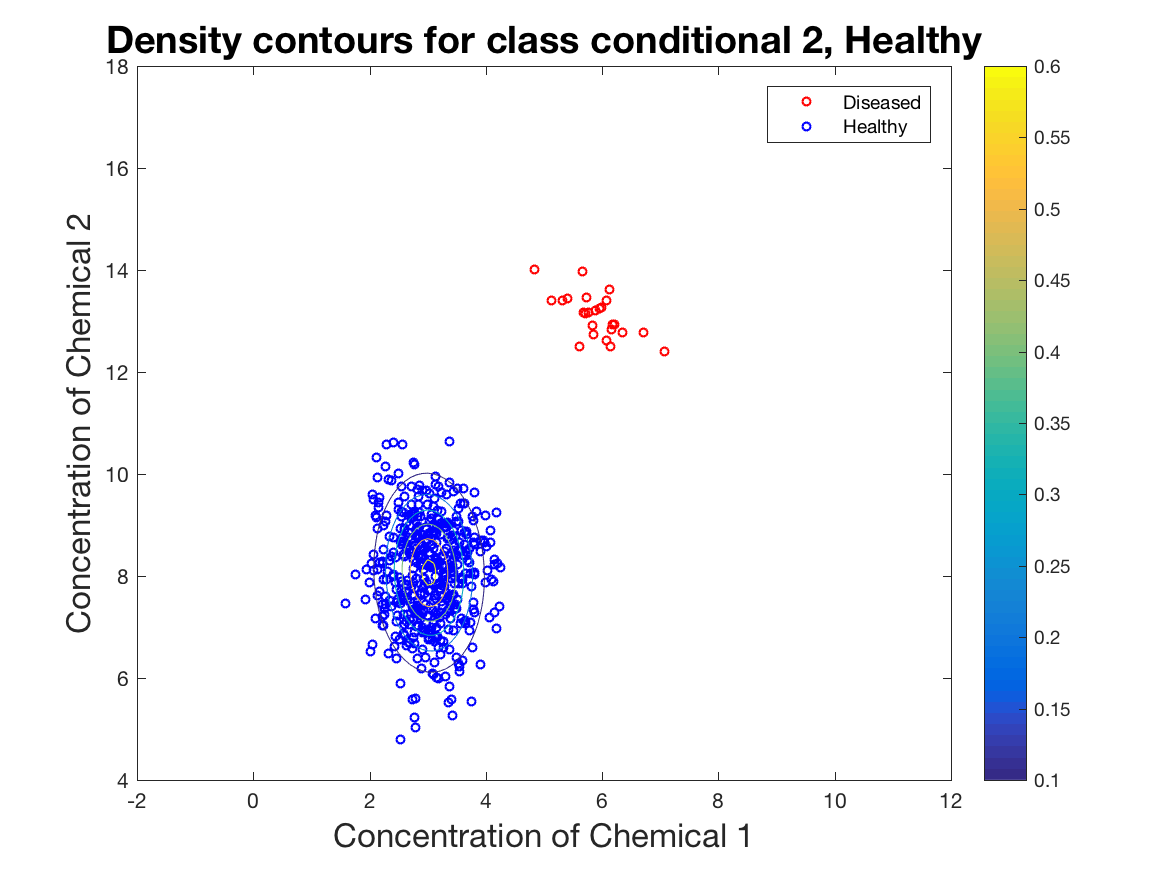
\includegraphics[width=\textwidth]{MLWONclassCondContoursHealthy.png}
		\caption{Polynomial model with order \textbf{n} = 3}
		\label{fig:model3}
	\end{subfigure}
	\caption{The original Olympic men's 400m data (blue crosses) with the polynomial models (red) overlaid.}
	\label{men400-1}
\end{figure}

\begin{figure}[h!] 
	\centering
	\begin{subfigure}[b]{0.4\textwidth}
		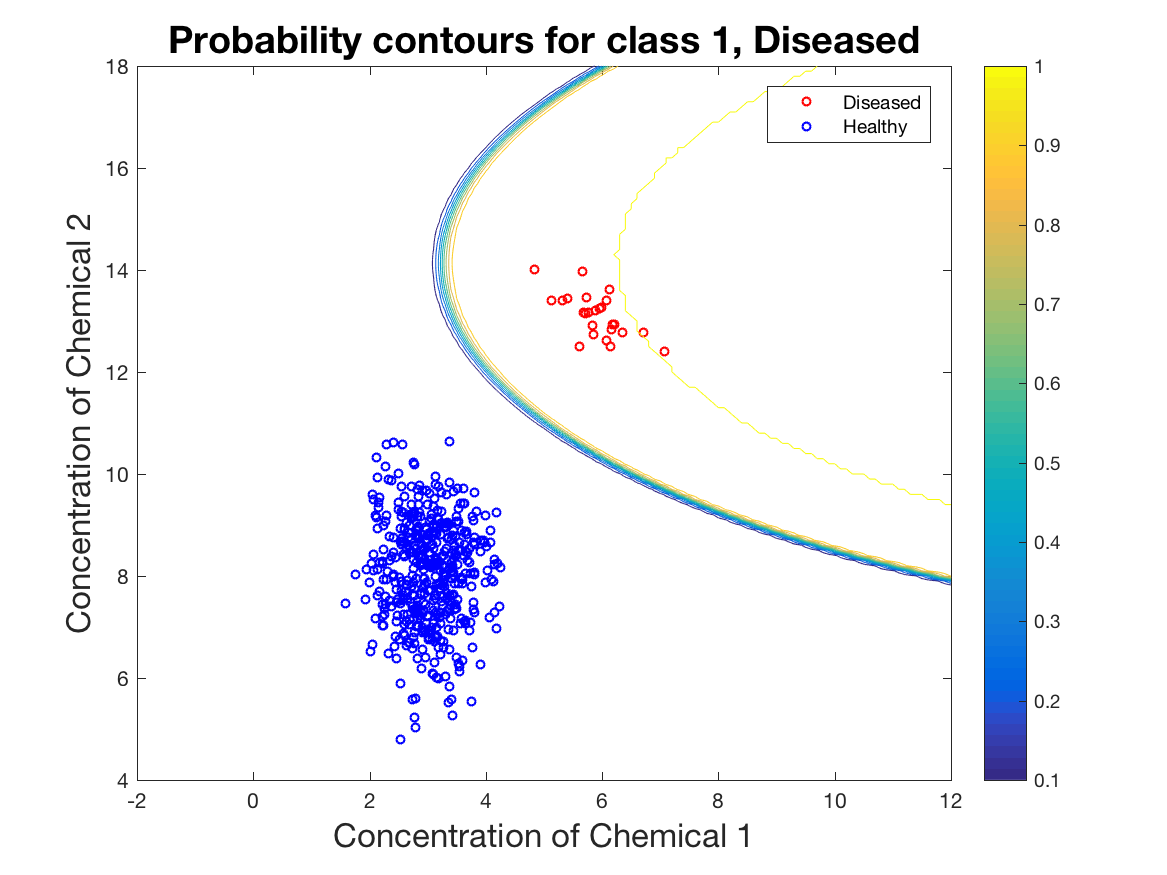
\includegraphics[width=\textwidth]{MLprobContoursDiseased.png}
		\caption{Polynomial model with order \textbf{n} = 0}
		\label{fig:model0}
	\end{subfigure}
	\begin{subfigure}[b]{0.4\textwidth}
		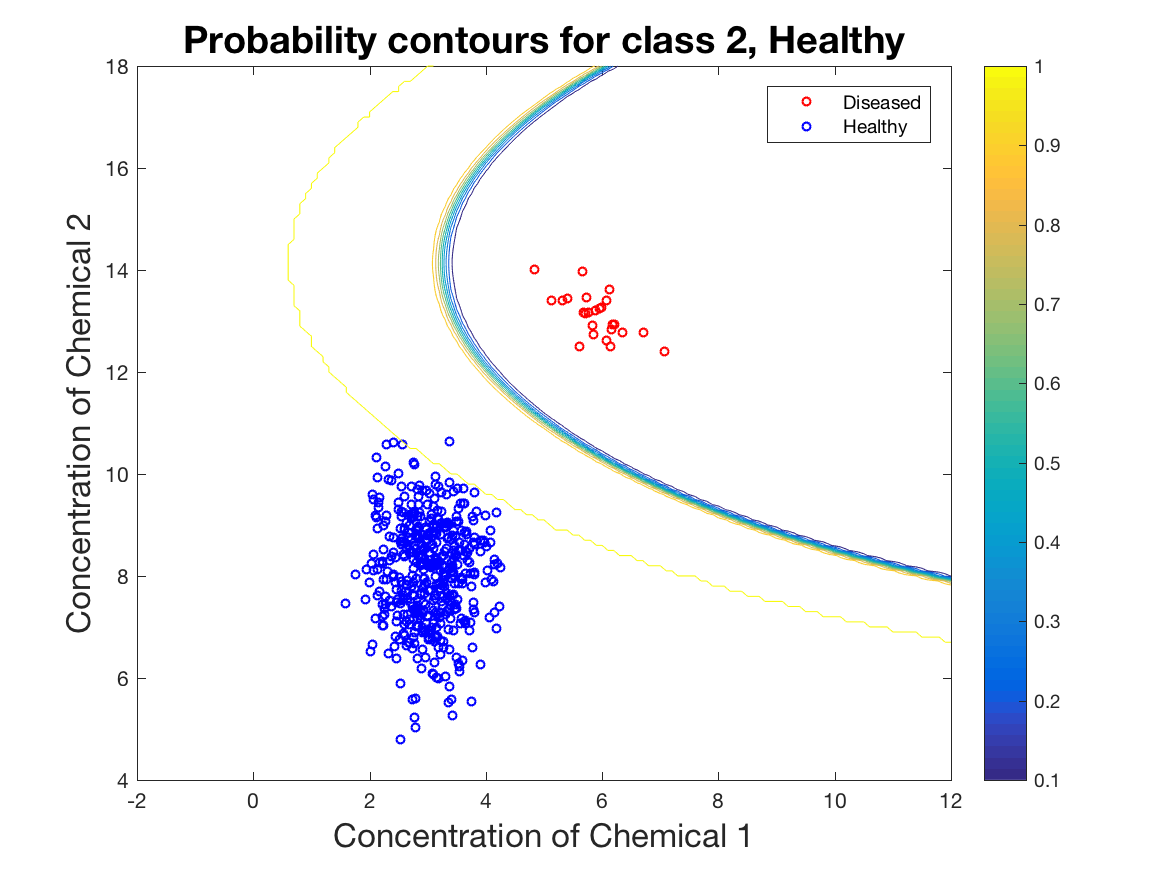
\includegraphics[width=\textwidth]{MLprobContoursHealthy.png}
		\caption{Polynomial model with order \textbf{n} = 1}
		\label{fig:model1}
	\end{subfigure}
	\begin{subfigure}[b]{0.4\textwidth}
		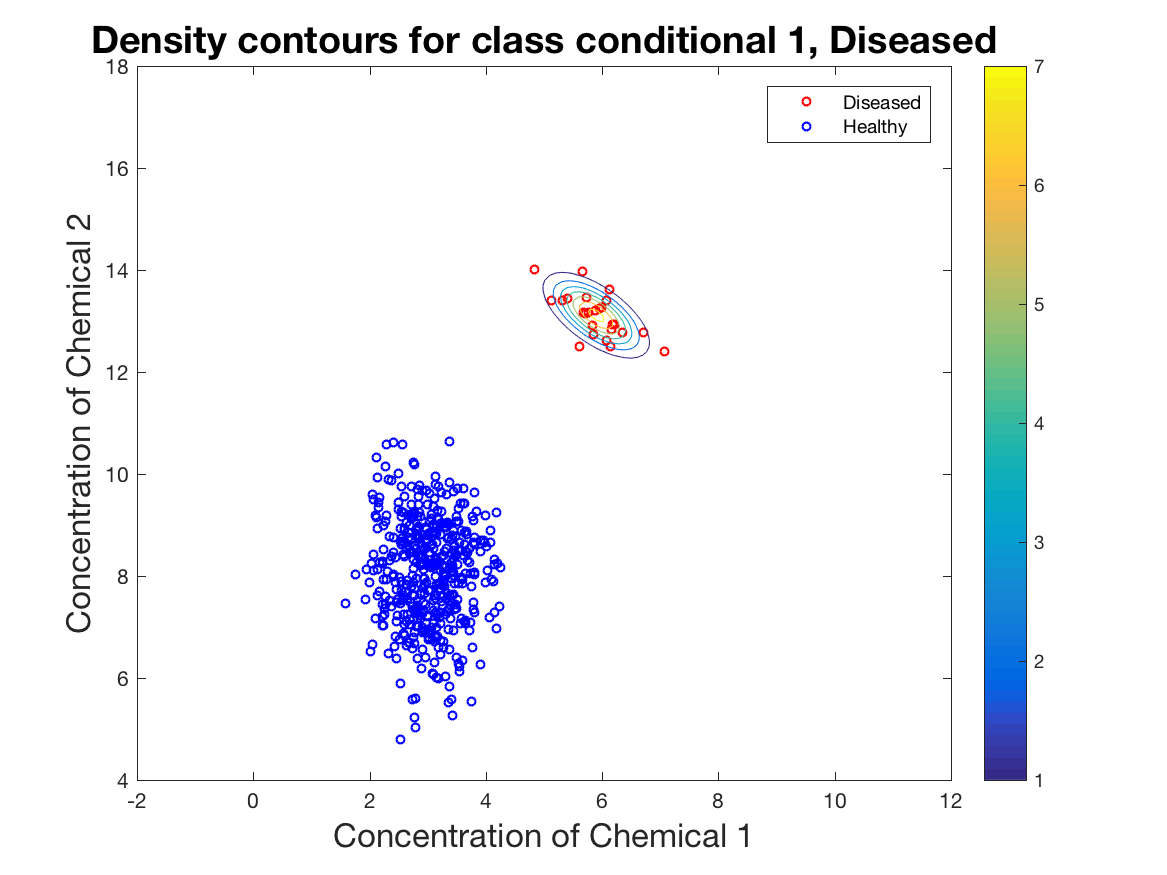
\includegraphics[width=\textwidth]{MLWONclassCondContoursDiseased.png}
		\caption{Polynomial model with order \textbf{n} = 2}
		\label{fig:model2}
	\end{subfigure}
	\begin{subfigure}[b]{0.4\textwidth}
		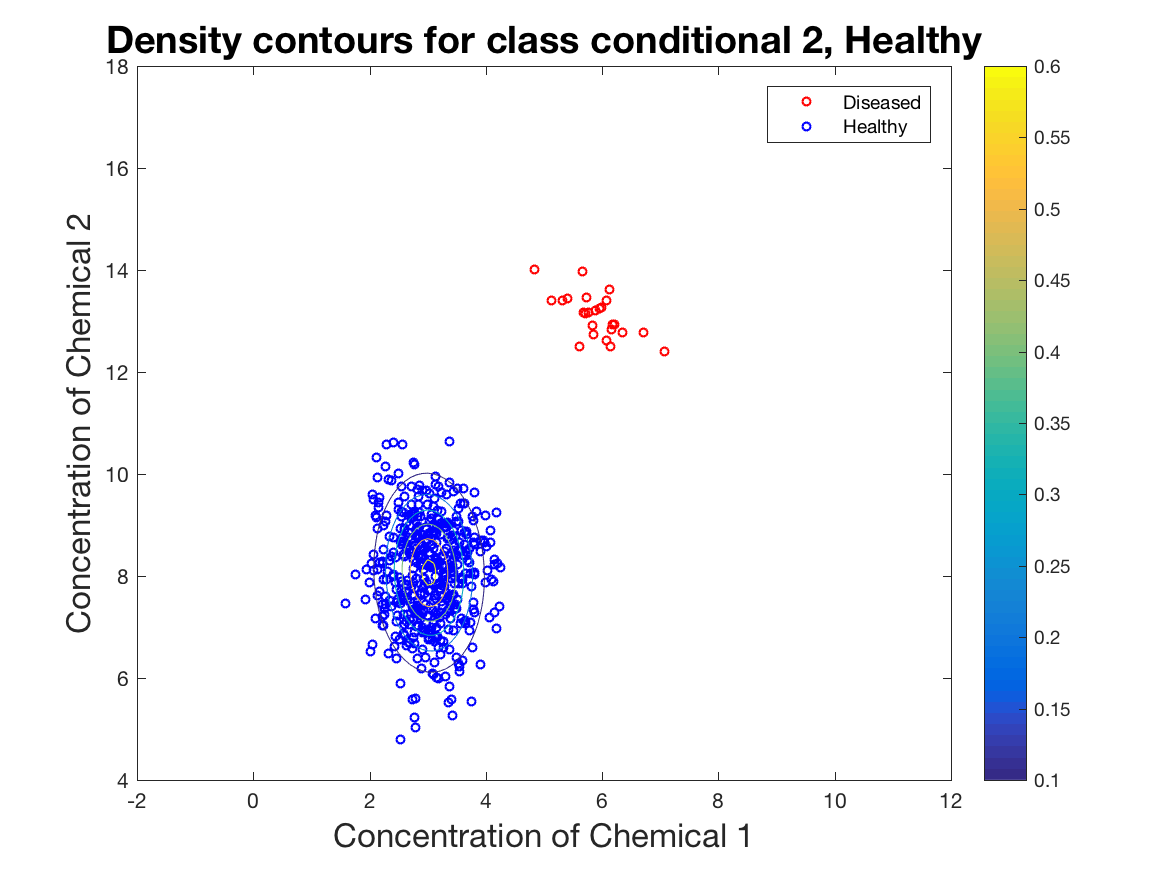
\includegraphics[width=\textwidth]{MLWONclassCondContoursHealthy.png}
		\caption{Polynomial model with order \textbf{n} = 3}
		\label{fig:model3}
	\end{subfigure}
	\caption{The original Olympic men's 400m data (blue crosses) with the polynomial models (red) overlaid.}
	\label{men400-1}
\end{figure}

Another point worth mentioning is the effect of permuting (randomising) the attributes. For this small dataset the permutations caused some instability in the model and different results were obtained as can be seen in Figure \ref{men400CVRandSt}. The results of the permuted data agree with the results from before.

\newpage
\section{Maximum A Posteriori (MAP)}{\label{s1}
	
	\subsection{Introduction}\label{Int}
	In Task 1, we are asked to analyse the Olympics men's 400m data. We must find the polynomial function of order \textbf{n} which best fits this data, where \textbf{n} is 1 to 4, and use 10-fold cross-validation to choose the "best" value of \textbf{n}. Refer to Appendix A for the Matlab code used for analysis.
	
	To compute the average cross validation loss, data (attributes and labels) are separated into 10 partitions (i.e. 10-fold), where 1 partition is reserved for testing the model. The 9 remaining partitions are used to learn the model with parameters, $w_{n}$. This models can use the attributes of the test partition to predict the labels, in this case the time ran for the men's 400m. The predicted values can then be compared to the actual values (labels)  from the test partition. The cross validation (CV) loss is calculated by taking the mean squared difference ($msd$) of these two values. This is then repeated 9 more times by rotating the test partition through. The average of these 10 $msd$ values is calculated and then plotted against the order to find the minimum value.
	
	\subsection{Results}\label{CVcons}
	From Figure \ref{fig:CVT4} and Table \ref{t:ModLoss} it is shown that a polynomial function with order 4 is the best fit. However, in order to determine the "best" order, it must be given a concrete meaning for this task. "Best" is considered to be the minimum mean squared loss, where loss is the difference between predicted and observed labels. Ideally, both cross-validation (CV) and training loss are considered but that is not always the case. So, three cases are defined as the following.
	
	\begin{enumerate}
		\item Only CV loss is considered
		\item Only Train loss is considered
		\item Both CV and Train loss are considered
	\end{enumerate}
	
	\begin{figure}[h]
		\centering
		\includegraphics[width=0.8\linewidth]{images/MAPnewData}
		\caption{Comparison of the CV and Train loss for polynomial models of order \textbf{n}, where \textbf{n} = 0 to 4.}
		\label{fig:CVT4}
	\end{figure}
	
	\begin{figure}[h]
		\centering
		\includegraphics[width=0.8\linewidth]{images/MAPWONnewData}
		\caption{Comparison of the CV and Train loss for polynomial models of order \textbf{n}, where \textbf{n} = 0 to 4.}
		\label{fig:CVT4}
	\end{figure}
	
	\begin{table}[h]
		\centering
		\caption{Classification Differences between Methods}
		\label{t:ModLoss}
		\begin{tabular}{rrrr}
			\hline
			\textbf{Order} & \textbf{CV Loss} & \textbf{Train Loss} & \textbf{Average Squared Loss} \\ \hline
			0 & 10.83 & 8.07 & 178.61 \\
			1 & 2.71 & 1.54 & 9.03 \\
			2 & 1.57 & 1.01 & 3.33 \\
			3 & 3.99 & 0.98 & 12.35 \\
			4 & 1.64 & 0.93 & 3.30
		\end{tabular}
	\end{table}
	
	Consider item 1, Figure \ref{fig:CVT4} and Table \ref{t:ModLoss} show that a polynomial function with order 2 is the best fit. It is visualised clearly on Figure \ref{fig:CVT4} as the minimum point on the line. Looking at Table \ref{t:ModLoss}, a minimum value of 1.57 also corresponds with order 2.
	
	Consider item 2, Figure \ref{fig:CVT4} and Table \ref{t:ModLoss} show that a polynomial function with order 4 is the best fit. Figure \ref{fig:CVT4} shows a downward trend to the right, indicating that an order of 4 is indeed the best fit. Looking at Table \ref{t:ModLoss}, the minimum value, 3.30, also corresponds with an order of 4.
	
	Consider item 3, Figure \ref{fig:CVT4} and Table \ref{t:ModLoss} show that a polynomial function with order 4 is the best fit. It is difficult to see this via the visualisation of Figure \ref{fig:CVT4}. However, looking at Table \ref{t:ModLoss}, the average squared loss (of CV and Train loss) is lowest when order equals 4. 
	
	Figure \ref{fig:model2} shows how well each of the models fit the data. Interestingly, Figure \ref{fig:model4}, shows an order of 4 provides an accurate model and more realistic future predictions than an order of 2. In comparison, an order of 2 shows that future predictions would increase in time at an increasing rate. This is highly unlikely given the downward trend of the data.
	
	The remaining models in Figure \ref{men400-1} clearly do not model the data well, where orders 1 and 3 show that a time of 0 will be achieved soon. This is not humanly possibly so the models can be discarded. 
	
	\subsection{Conclusion}
	The problem for Task 1 is to find the "best model based on average cross-validation loss." This only considers point 1 from before, therefore, a polynomial function with order 2 best fits the model based on average cross-validation loss.
	
	\begin{figure}[h!] 
		\centering
		\begin{subfigure}[b]{0.4\textwidth}
			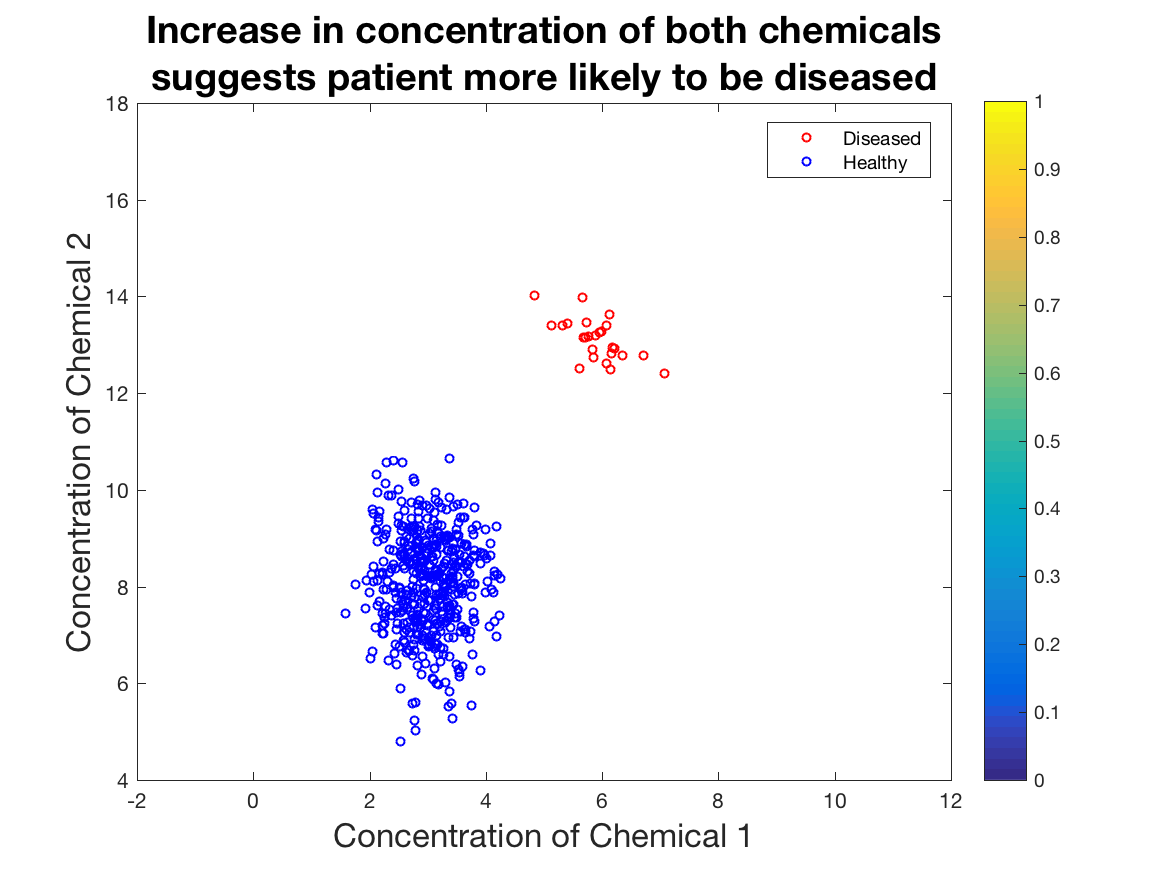
\includegraphics[width=\textwidth]{MAPtrainingData.png}
			\caption{Polynomial model with order \textbf{n} = 3}
			\label{fig:modelNoReg0}
		\end{subfigure}
		\begin{subfigure}[b]{0.4\textwidth}
			\includegraphics[width=\textwidth]{MAPnewData.png}
			\caption{Polynomial model with order \textbf{n} = 4}
			\label{fig:modelNoReg1}
		\end{subfigure}
		\begin{subfigure}[b]{0.4\textwidth}
			\includegraphics[width=\textwidth]{MAPWONnewData.png}
			\caption{Polynomial model with order \textbf{n} = 4}
			\label{fig:modelNoReg1}
		\end{subfigure}
		\caption{The original Olympic men's 400m data (blue crosses) with the polynomial models (red) overlaid without data standardisation.}
		\label{men400-1noSt}
	\end{figure}
	
	\subsection{Further Comments}
	Further investigation found if the data was not standardised, a systematic error is produced in the model for orders greater than or equal 4. Figure \ref{men400-1noSt} illustrates an order of 3 produces no error, but an order of 4 does. Reviewing literature showed this systematic error is common when dealing with high order polynomial function\cite{WhenIsIt}.Therefore, it is good practice to standardise data when the regression model contains polynomial terms.
	
	\begin{figure}[h!] 
		\centering
		\begin{subfigure}[b]{0.4\textwidth}
			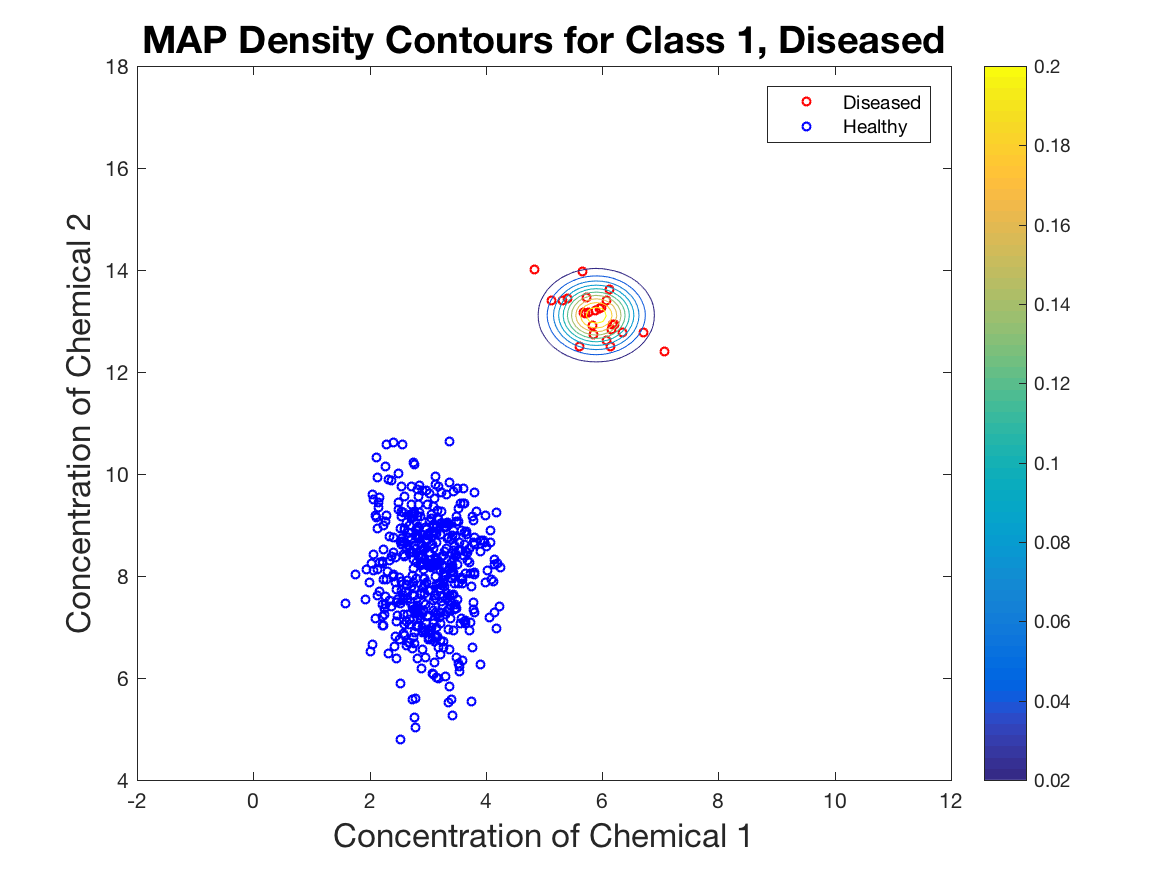
\includegraphics[width=\textwidth]{MAPclassCondContoursDiseased.png}
			\caption{Polynomial model with order \textbf{n} = 0}
			\label{fig:model0}
		\end{subfigure}
		\begin{subfigure}[b]{0.4\textwidth}
			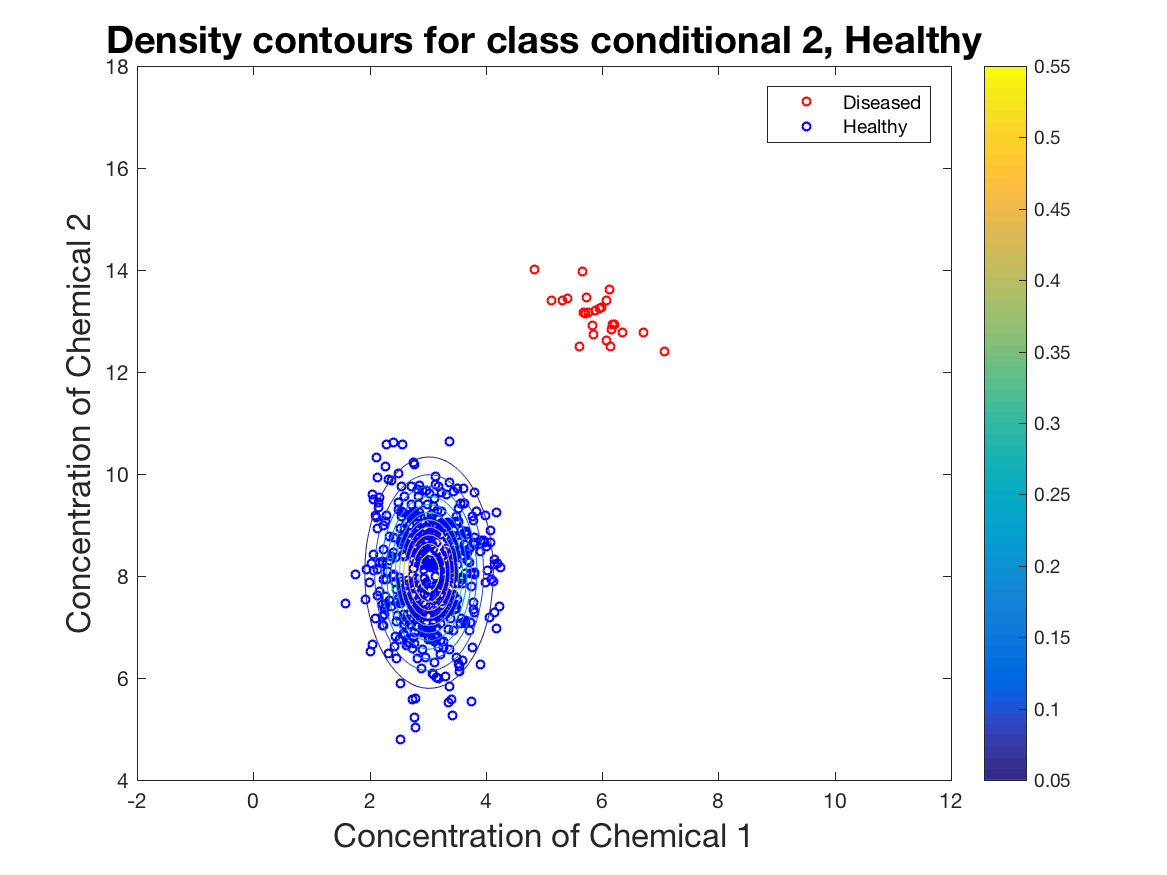
\includegraphics[width=\textwidth]{MAPclassCondContoursHealthy.png}
			\caption{Polynomial model with order \textbf{n} = 1}
			\label{fig:model1}
		\end{subfigure}
		\begin{subfigure}[b]{0.4\textwidth}
			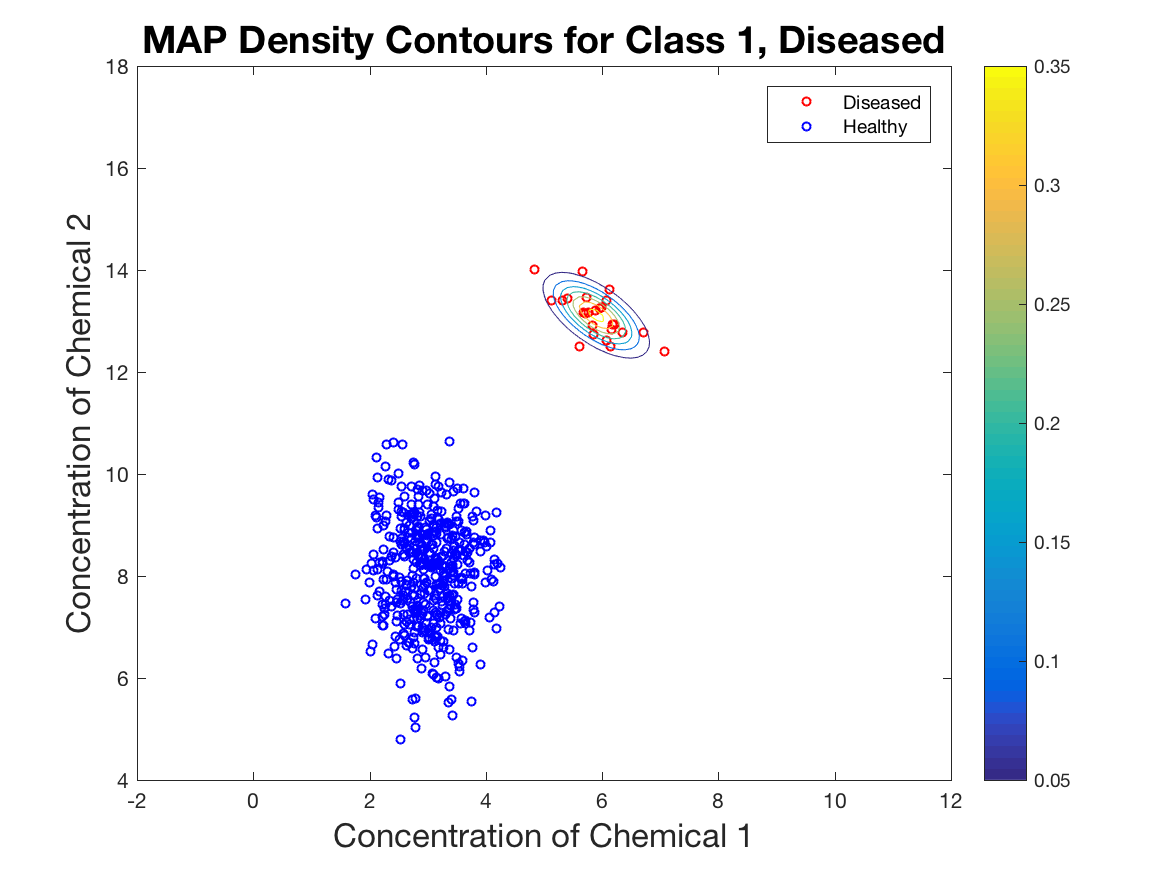
\includegraphics[width=\textwidth]{MAPWONclassCondContoursDiseased.png}
			\caption{Polynomial model with order \textbf{n} = 2}
			\label{fig:model2}
		\end{subfigure}
		\begin{subfigure}[b]{0.4\textwidth}
			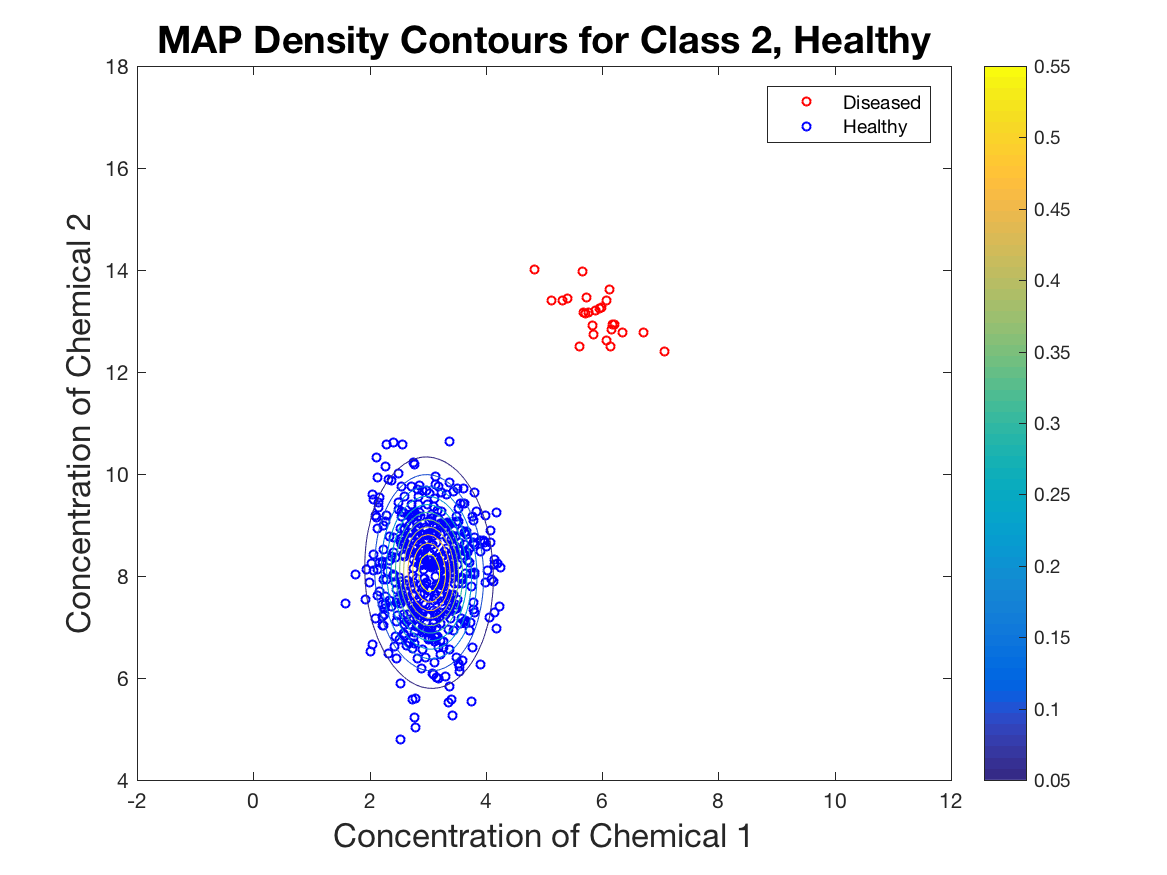
\includegraphics[width=\textwidth]{MAPWONclassCondContoursHealthy.png}
			\caption{Polynomial model with order \textbf{n} = 3}
			\label{fig:model3}
		\end{subfigure}
		\caption{The original Olympic men's 400m data (blue crosses) with the polynomial models (red) overlaid.}
		\label{men400-1}
	\end{figure}
	
	\begin{figure}[h!] 
		\centering
		\begin{subfigure}[b]{0.4\textwidth}
			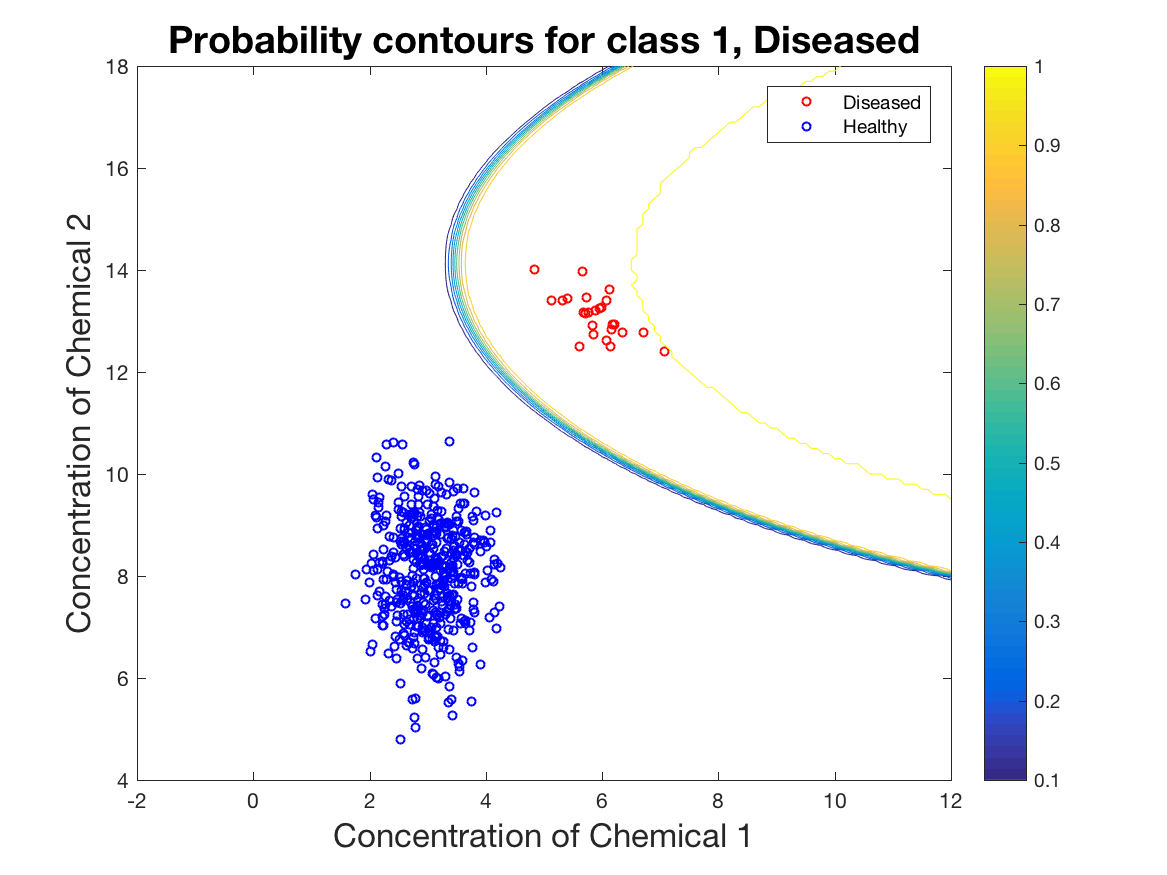
\includegraphics[width=\textwidth]{MAPprobContoursDiseased.png}
			\caption{Polynomial model with order \textbf{n} = 0}
			\label{fig:model0}
		\end{subfigure}
		\begin{subfigure}[b]{0.4\textwidth}
			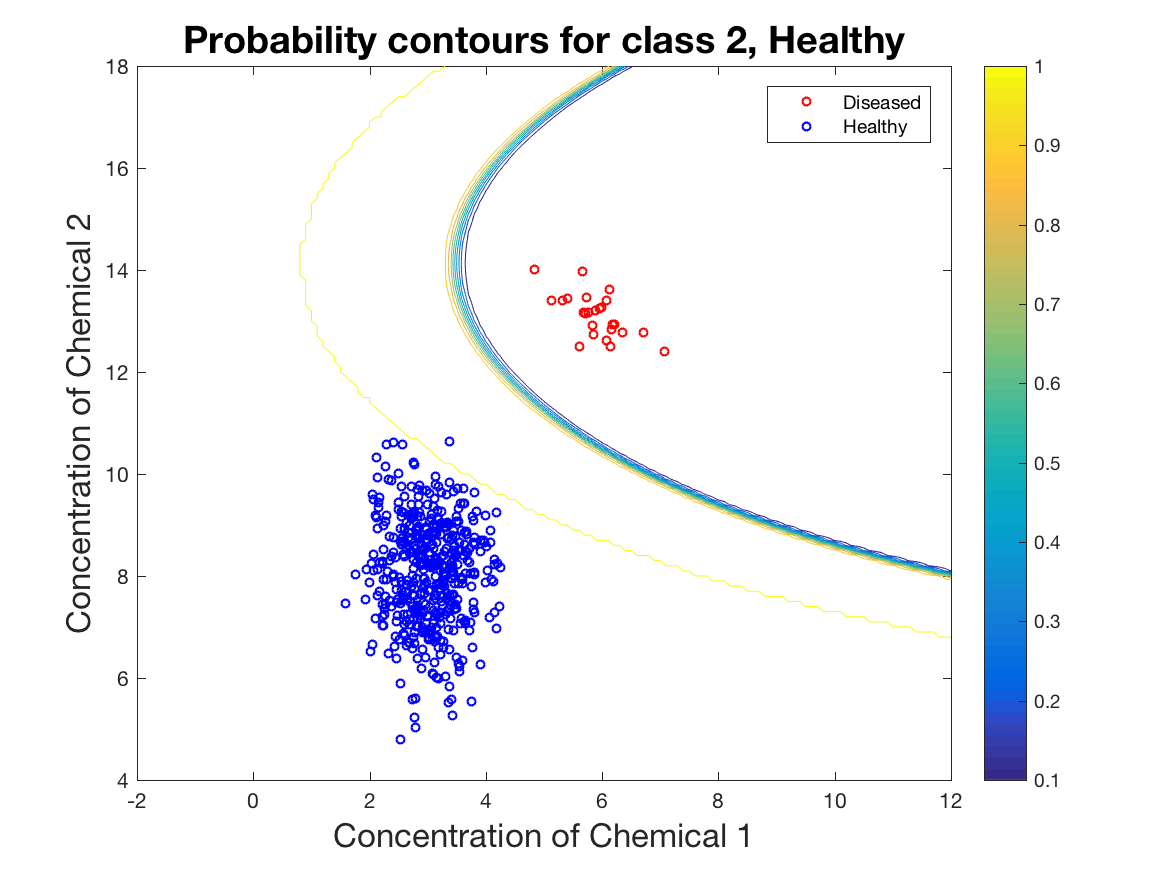
\includegraphics[width=\textwidth]{MAPprobContoursHealthy.png}
			\caption{Polynomial model with order \textbf{n} = 1}
			\label{fig:model1}
		\end{subfigure}
		\begin{subfigure}[b]{0.4\textwidth}
			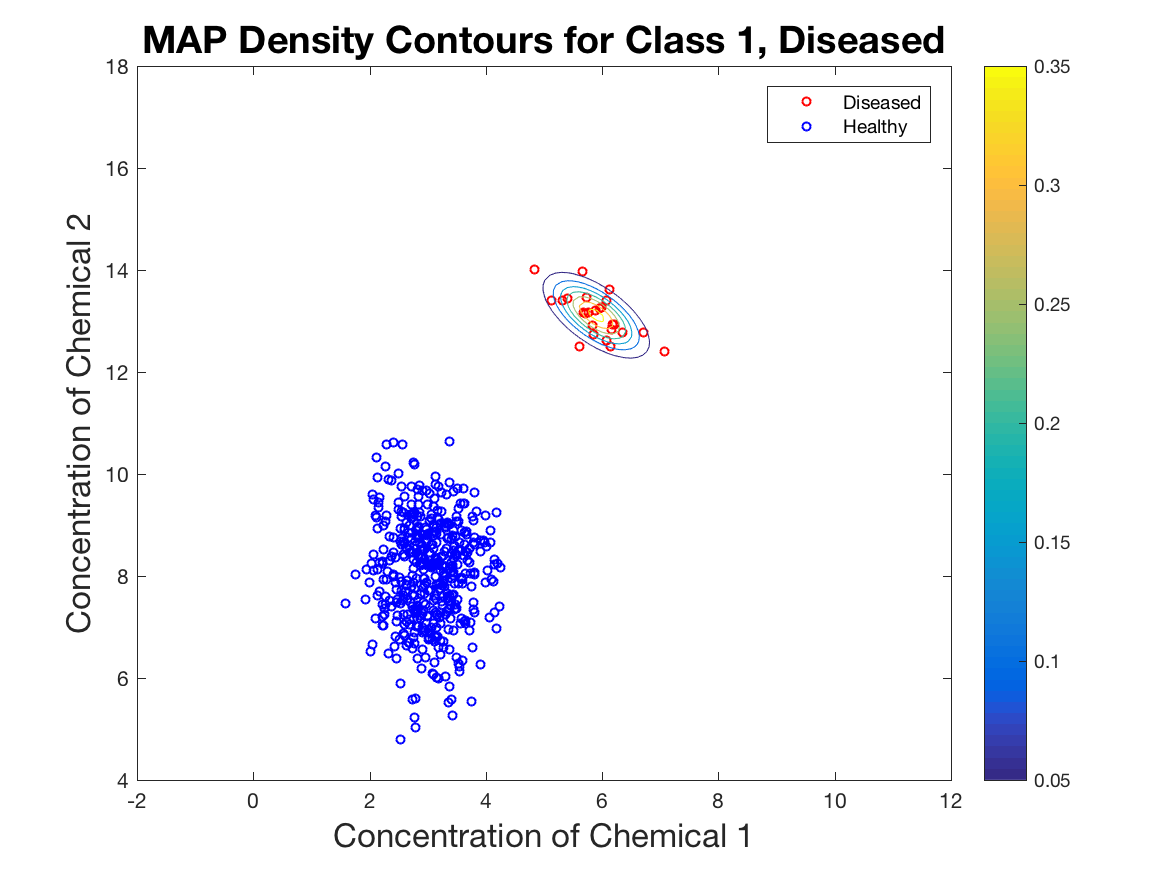
\includegraphics[width=\textwidth]{MAPWONclassCondContoursDiseased.png}
			\caption{Polynomial model with order \textbf{n} = 2}
			\label{fig:model2}
		\end{subfigure}
		\begin{subfigure}[b]{0.4\textwidth}
			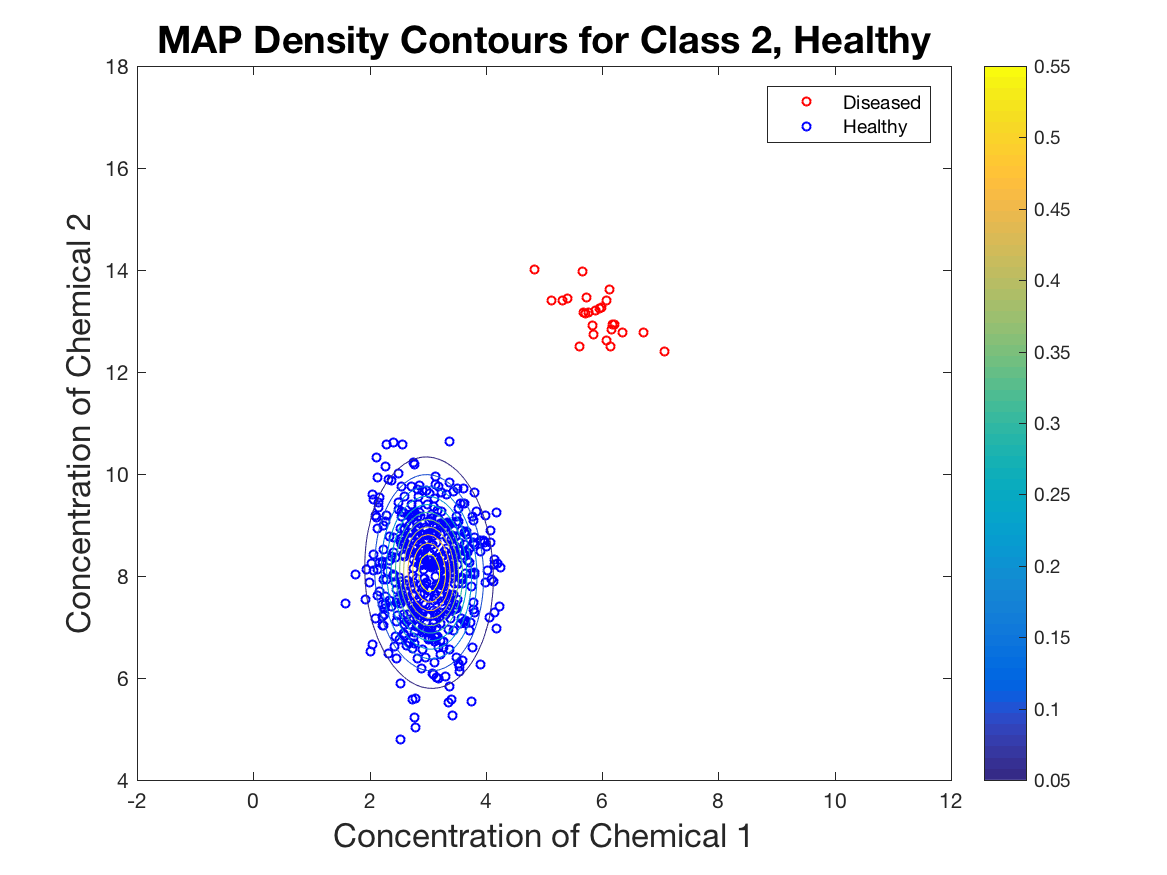
\includegraphics[width=\textwidth]{MAPWONclassCondContoursHealthy.png}
			\caption{Polynomial model with order \textbf{n} = 3}
			\label{fig:model3}
		\end{subfigure}
		\caption{The original Olympic men's 400m data (blue crosses) with the polynomial models (red) overlaid.}
		\label{men400-1}
	\end{figure}
	
	Another point worth mentioning is the effect of permuting (randomising) the attributes. For this small dataset the permutations caused some instability in the model and different results were obtained as can be seen in Figure \ref{men400CVRandSt}. The results of the permuted data agree with the results from before.
	
\newpage	
\section{Maximum Likelihood vs Maximum A Posteriori  \\ (ML VS MAP)}{\label{s1}
	
	\subsection{Difference of ML and MAP}\label{Int}
	In Task 1, we are asked to analyse the Olympics men's 400m data. We must find the polynomial function of order \textbf{n} which best fits this data, where \textbf{n} is 1 to 4, and use 10-fold cross-validation to choose the "best" value of \textbf{n}. Refer to Appendix A for the Matlab code used for analysis.
	
	To compute the average cross validation loss, data (attributes and labels) are separated into 10 partitions (i.e. 10-fold), where 1 partition is reserved for testing the model. The 9 remaining partitions are used to learn the model with parameters, $w_{n}$. This models can use the attributes of the test partition to predict the labels, in this case the time ran for the men's 400m. The predicted values can then be compared to the actual values (labels)  from the test partition. The cross validation (CV) loss is calculated by taking the mean squared difference ($msd$) of these two values. This is then repeated 9 more times by rotating the test partition through. The average of these 10 $msd$ values is calculated and then plotted against the order to find the minimum value.
	
		\subsection{Affects of Difference on this Data}\label{Int}
	In Task 1, we are asked to analyse the Olympics men's 400m data. We must find the polynomial function of order \textbf{n} which best fits this data, where \textbf{n} is 1 to 4, and use 10-fold cross-validation to choose the "best" value of \textbf{n}. Refer to Appendix A for the Matlab code used for analysis.
	
	To compute the average cross validation loss, data (attributes and labels) are separated into 10 partitions (i.e. 10-fold), where 1 partition is reserved for testing the model. The 9 remaining partitions are used to learn the model with parameters, $w_{n}$. This models can use the attributes of the test partition to predict the labels, in this case the time ran for the men's 400m. The predicted values can then be compared to the actual values (labels)  from the test partition. The cross validation (CV) loss is calculated by taking the mean squared difference ($msd$) of these two values. This is then repeated 9 more times by rotating the test partition through. The average of these 10 $msd$ values is calculated and then plotted against the order to find the minimum value.
	
	Insert Table showing difference!!!
